\documentclass{article}

\usepackage{amsmath, tikz}
\usepackage[version=4]{mhchem}
\usetikzlibrary{positioning}
\title {Cambridge GCSE Notes \\ 5070 Chemistry }
\author {Abrar Faiyaz Rahim, degrees pending}
\date {}
\renewcommand*{\thefootnote}{[\arabic{footnote}]}
\begin{document}
\maketitle \newpage
\tableofcontents

\section{Electrochemistry}
\subsection{Electrolysis}

Electrolysis is the decomposition of an ionic compound, in molten or aqueous form, by passage
of electric current.

A simple electrolytic cell consists of two electrodes, the cathode and anode, connected to either
side of a battery and an electrolyte. The anode is positively charged whereas the cathode is
negatively charged. The electrolyte is the aqueous or molten substance that undergoes decomposition
through electrolysis.

In the external circuit consisting of wires connected to the batteries, electrons flow from the
battery to the cathode, making the cathode negatively charged. Here electrons are lost to 
substances in the electrolyte which are oxidised. The anode, being positively charged, attracts
the negative ions from the ionic compound, oxidising them, by taking their
excess electrons electrons. Electrons are
gained at the anode from negative ions, and are lost at the cathode to positive ions. The 
electrodes can be made of any conductive material, such as metals or graphite. Graphite electrodes
are said to be inert as they do not take part in the reaction. Note that, oxidation occurs at
anodes and reduction occurs at cathodes.

In case of the substance, lead (II) bromide, \ce{PbBr2}, the following happens 
during electrolysis with inert electrodes
at either electrode:

\begin{center}
at anode: \ce{2Br- -> Br2 + 2e-}

at cathode: \ce{Pb$^{2+}$ + 2e- -> Pb}
\end{center}

It is observed that a silvery solid accumulates at the cathode, i.e. lead (II) and a red-brown
gas is given off at anode. Note that, from here we can judge that for molten ionic compounds, the
metal part of the compound will always form at the cathode, and the non metal will form at the
anode.

During electrolysis of concentrated aqueous sodium chloride, using inert electrodes, the following
reactions occur at the electrodes:
\begin{center}
	at anode: \ce{2Cl- -> Cl2 + 2e-}

	at cathode: \ce{H+ + 2e- -> H2}
\end{center}
It is observed that a colourless gas is given off at cathode and a green gas is given off at the
anode.

The reason why the metal, i.e., sodium is not discharged at the cathode is because it is not the
least reactive amongst the cations present in the electrolyte. The ions present in the electrolyte
are: \ce{H+}, \ce{Na+}, \ce{Cl-} and \ce{OH-}. Of these, at the cathode the ion discharged is
the least reactive of the cations, and at the anode the ion discharged is the ion that loses 
electrons more readily, and is hence easier to discharge. The reactivity series of cations and
the prefential discharge rule of anions are given below:

$$\ce{Na+} > \ce{Mg^{2+}} > \ce{Al^{3+}} > \ce{Zn^{2+}} > \ce{H+} > \ce{Cu^{2+}} > \ce{Ag+} \footnote{where the ion to the left of $>$ is more reactive than the ion to the right.
}$$
$$ \ce{SO4^{2-}} < \ce{NO3^{-}} < \ce{OH-} < \ce{Cl-} < \ce{Br-} < \ce{I-} \footnote{where the
ion to the left of $<$ is less likely to be discharged than that to the right.}$$

During the electrolysis of dilute sulfuric acid, the ions in the electrolyte are: \ce{H+}, \ce{OH-},
\ce{SO4$^{2-}$}. The only cation, \ce{H+} is released at the cathode and, by preferential rule,
\ce{OH-} is the one which is oxidised at anode.
\begin{center}
	at cathode: \ce{2H+ + 2e- -> H2}

	at anode: \ce{4OH- -> O2 + 2H2O + 4e-}
\end{center}
Colourless gases are given off at both electrodes, but the volume of oxygen produced is half that
of hydrogen. This is a result of the fact that, the mole ratio of oxygen to hydrogen in the 
electrolyte is 1:2.

Consider the case of the electrolysis of aqueous copper (II) sulfate using inert electrodes. 
Uncharged copper (\ce{Cu}) has a pinkish-orange colour, whereas copper ions, \ce{Cu$^{2+}$} have
a blue colour. The following happens at the electrodes in this electrolysis:
\begin{center}
	at cathode: \ce{Cu$^{2+}$ + 2e- -> Cu}

	at anode: \ce{OH- -> O2 + 2H2O + 4e-}
\end{center}
Notice that, the copper ions are reduced to copper, reducing the number of copper ions in 
electrolyte. It is observed that the blue colour of solution fades and a pinkish orange solid
accumulates on the cathode.

An active electrode is that which takes part in the electrolytic process. Consider the case
of the electrolysis of aqueous copper (II) sulfate with copper electrodes. It is seen that copper
deposites on the cathode and copper is dissolved at the anode.
\begin{center}
	at cathode: \ce{Cu$^{2+}$ + 2e- -> Cu}

	at anode: \ce{Cu -> Cu$^{2+}$ +  2e-}
\end{center}

This property of active electrodes and metals comes in use during electroplating, which is a
process of electrolysis in which a metal object is coated/plated with a layer of another metal.

To electroplate a metal object, we must place it as the cathode, and have the anode be the metal with
which we want to plate the metal object. The electrolyte must be the solution of a salt with the
metal to plate with.

\subsection{Hydrogen-oxygen fuel cells}

It is possible to use chemical reactions to produce electrical energy. Everyday batteries work in
this way. A more efficient method would be using a fuel cell. A hydrogen oxygen fuel cell uses
the following chemical reaction

\begin{center}
	\ce{2H2(g) + O2(g) -> 2H2O(l)}
\end{center}
Here, the hydrogen is considered to be a non-polluting fuel. 

As a fuel, hydrogen is more efficient than any other, and the only waste product formed is water.
However, due to it being difficult to produce and unsafe to store, it has failed to gain precedence.

\section{Chemical energetics}
\subsection{Exothermic and endothermic reactions}

An exothermic reactions transfers thermal energy to the surroundings leading to an increase in the
temperature of the surroundings. An endothermic reaction takes in thermal energy from the 
surroundings leadin gto a decrease in the temperature of the surroundings.

The transfer of energy during a reaction is caleed the enthalpy change, $\Delta H$ of the reaction.
The value is negative for exothermic reactions and positive for endothermic reactions.

Activation energy, $E_a$ is the minimum energy that colliding particles must have to react.
\begin{center}
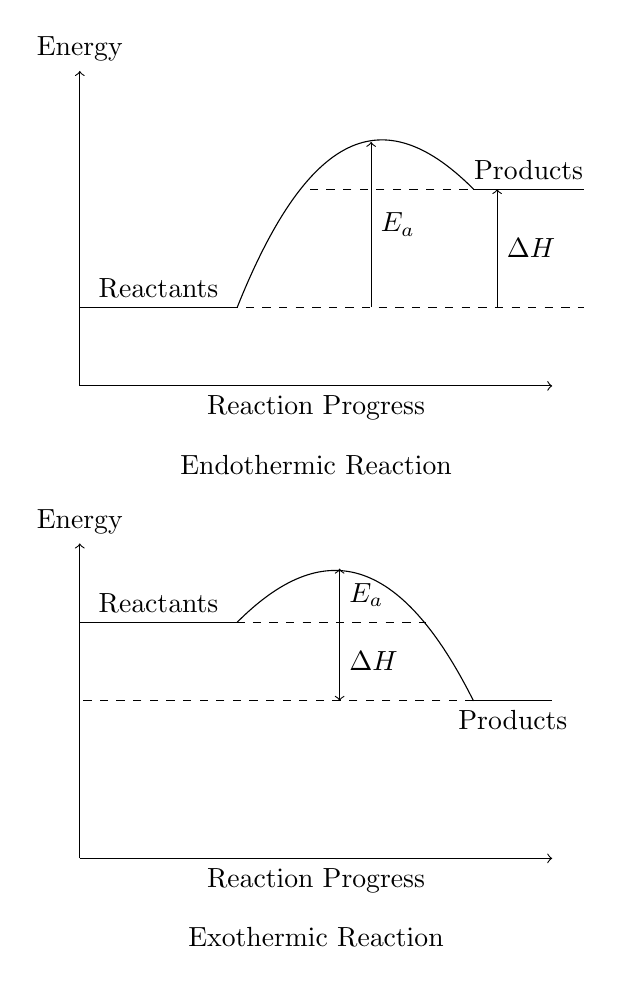
\begin{tikzpicture}

    % Axes for Endothermic Reaction
    \draw[->] (0,0) -- (6,0) node[below, midway] {Reaction Progress};
    \draw[->] (0,0) -- (0,4) node[above] {Energy};

    % Reactants for Endothermic
    \draw (0,1) -- (2,1) node[above, midway] {Reactants};
	\draw[dashed] (0, 1) -- (6.4, 1);

    % Activation energy curve for Endothermic
    \draw (2,1) .. controls (3,3.5) and (4,3.5) .. (5,2.5);

    % Products for Endothermic
    \draw (5,2.5) -- (6.4,2.5) node[above, midway] {Products};
	\draw[dashed] (6.4, 2.5) -- (2.8, 2.5);

    % Activation energy arrow for Endothermic
    \draw[->] (3.7,1) -- (3.7,3.1) node[midway,right] {$E_a$};

    % Enthalpy change arrow for Endothermic
    \draw[->] (5.3,1) -- (5.3,2.5) node[midway,right] {$\Delta H$};

    % Label Endothermic
    \node at (3,-1) {Endothermic Reaction};

    % Axes for Exothermic Reaction (below)
    \draw[->] (0,-6) -- (6,-6) node[below, midway] {Reaction Progress};
    \draw[->] (0,-6) -- (0,-2) node[above] {Energy};

    % Reactants for Exothermic
    \draw (0,-3) -- (2,-3) node[above, midway] {Reactants};

    % Activation energy curve for Exothermic
    \draw (2,-3) .. controls (3,-2) and (4,-2) .. (5,-4);

    % Products for Exothermic
    \draw (5,-4) -- (6,-4) node[midway, below] {Products};

    % Activation energy arrow for Exothermic
    \draw[->] (3.3,-3) -- (3.3,-2.32) node[midway,right] {$E_a$};
	\draw[dashed] (0.3, -3) -- (4.4, -3);

    % Enthalpy change arrow for Exothermic
    \draw[<-] (3.3,-4) -- (3.3,-3) node[midway,right] {$\Delta H$};
	\draw[dashed] (5, -4) -- (0, -4);

    % Label Exothermic
    \node at (3,-7) {Exothermic Reaction};

\end{tikzpicture}
\end{center}
Above are reaction pathway diagrams, showing the energy of a reaction as it progresses. The
energy of products is greater than that of the reactants in endothermic reactions and the opposite
is true for exothermic reactions. The differences in energy and their correspondences are labelled.

Remember that M-EXO (making is exo) and B-ENDO (breaking is endo).

Bond breaking is an endothermic process and bond making is an exothermic process. When a reaction,
overall, has bonds broken with more energy than bonds made, it is endothermic. The opposite is
also applies.

Enthalpy change can be calculated as:
\begin{center}
	enthalpy = (energy needed to break bonds) - (energy needed to
	make bonds)
\end{center}
\[\Delta H = E_b - E_f\]
where $E_b$ is the energy needed to break bonds and $E_f$ is that needed to form bonds.

\section{Chemical reactions}
\subsection{Physical and chemical changes}
In a physical change, the substances present remain chemically the same and no new substances
are formed. Such changes are often easy to reverse.

Changes such as melting and boiling are endothermic as heat is taken in, changes such as 
condensing and freezing are exothermic as heat is given out.

Chemical changes are those where a new substances is formed. Most chemical changes happen through
chemical reactions, almost all of which are exothermic, very few are endothermic.

\subsection{Rate of reaction}
A reaction progresses when effective collisions occur between reactants to form a molecule of a
product. The rate of effective collisions is hence the rate of the reaction. This rate of effective
collisions can be influenced. These effective collisions can only occur if the colliding particles
have a minimum energy ($E_a$).

Increasing the number of particles per unit volume means there are more particles per unit volume,
when that is the case the particles are more likely to react.

Increasing the kinetic energy (KE) of particles by applying heat makes them move faster, meaning
more particles are likely to collide more frequently and with energy greater that $E_a$.

A catalyst is that which increases the rate of a reaction, decreases the $E_a$ and is unchanged
at the end of the reaction.

Changing solution concentration changes particles per unit volume, refer above.

Changing gas pressure does the same, refer above.

Increasing surface area of solids means there are more exposed surfaces with which reactants can
effectively collide, meaning effective collisions are more likely. The opposite is also true.

Increasing temperature increases KE of particles, refer above.

Addition of a catalyst, including enzymes, increases reaction rate and decreases $E_a$.

Investigating the rate of a reactioon comes down to measuring the rate at which reactants are used
up or the rate at which products are formed. The information can be represented in a graph:

\begin{center}
\begin{tikzpicture}
    % Axes
    \draw[->] (0,0) -- (6,0) node[right] {Time};
    \draw[->] (0,0) -- (0,4) node[above] {Loss in Mass};

    % Curve A (slower and levels off later)
    \draw[thick] (0,0) .. controls (2,2.5) and (4,3.2) .. (5.5,3.5) node[below, midway] {A};

    % Curve B (faster and levels off earlier)
    \draw[thick,dashed] (0,0) .. controls (1,3) and (3,3.4) .. (5.5,3.5) node[above, midway] {B};
    
\end{tikzpicture}
\end{center}
In reaction B, the reactants were powdered, with increased surface area and hence the reaction had
a faster rate than A with just solid reactants. Notice that they loss in mass is equal but the rate
of loss of mass is the difference.

\subsection{Reversible reactions and equilibrium}
Most reactions are one-way, i.e., reactants react to form products and that's it. Some reactions,
are reversible, in such reactions, reactants react to form products and those products also react
to form reactants. Such reactions are shown with a ``$\rightleftharpoons$":

\begin{center}
	\ce{N$_2$(g) + 3H$_2$(g) <=>[forward reaction][backward reaction] 2NH$_3$(g)}
\end{center}

Changing the direction of a reversible reaction can depend on the conditions applied to it.
Such is the case for hydrating and making anhydrous salts.

\begin{center}
	\ce{CoCl2 * 6H2O <=>[heat][water] CoCl2 + 6H2O}

	\ce{CuSO4 * 6H2O <=>[heat][water] CuSO4 + 6H2O}
\end{center}

Note that, \ce{CuSO4} is white while the hydrated form \ce{CuSO4 * H2O} is blue. Hydrated cobalt (II)
chloride is pink whereas the anhydrous form is blue.

A closed system is that where no reactants or products can escape from the reacting system. In such
a system, a reversible reaction is in equilibrium when the rate of forward reaction equals the
rate of backward reaction and the concentrations of reactants and products are not changing. The
reagents are reacting but the concentrations do not change.

The position of equilibrium tells us the rate of forward reaction compared to backward reactions.
That means, if the position of equilibrium is to the right, the rate of forward reaction is greater
than that of the backward reaction and vice versa.

Note that, when a change is made to the conditions of a system in dynamic equilibrium, the system 
moves so as to oppose that change.

Changing temperature affects the reaction depending on the enthalpy of the reaction. Changing the
temperature will cause the equilibrium to shift in the direction that will reverse that change.
Increasing the temperature in a reaction where the forward reaction is exothermic will shift 
equilibrium to left, as the system will oppose the change by increasing rate of endothermic 
reaction to lower temperature. The opposite is also true.

Changing pressure only affects reactions whose reagents are all gaseous. Increasing pressure moves
equilibrium toward the side which has less gaseous moles. The opposite is also true.

Increasing concentration of reactants moves equilibrium to right and more products are formed and
vice versa.

Using a catalyst does not affect equilibrium position, but the speed at which the system reaches 
equilibrium is affected by catalyst.

Below is the symbol equation for the Haber process.
\begin{center}
	\ce{N2(g) + 3H2(g) <=>[450 $^{\circ}$C][200 atm] 2NH3(g)} $\Delta H < 0$
\end{center}
The nitrogen is gotten from fractional distillation of liquid air and hydrogen is gotten from 
cracking of crude oil. The above reaction requires an iron catalyst.

In the Contact process, sulfur dioxide is converted into sulfur trioxide.
\begin{center}
	\ce{2SO2(g) + O2(g) <=>[450 $^{\circ}$C][2 atm] 2SO3(g)} $\Delta H < 0$
\end{center}
The Contact process requires a vanadium (V) oxide, \ce{V2O5} catalyst. Sulfur dioxide is gotten
from burning or roasting sulfide ores:
\begin{center}
	\ce{S(s) + O2(g) -> SO2(g)} 
\end{center}
and oxygen is gotten from air.

The conditions in the above industrial processes are such that to optimise economical costs and
safety.

\subsection{Redox}
Roman numbers are used to indicate the oxidation number of an element in a compound (iron (II), 
vanadium (V), etc.).

A redox reaction is where reduction and oxidation occurs simultaneously.

The oxidation of a compound is its gain of oxygen, loss of electrons or increase in oxidation 
number.

The reduction of a compound is its loss of oxygen, gain of electrons or decrease in oxidation
number.

Rules for identifying oxidation number:
\begin{itemize}
	\item It is zero in uncombined states (B, Mg).
	\item It is the same as the charge on an ion (B$^{+2}$).
	\item Sum of oxidation numbers in a compound is zero.
	\item Sum of oxidation numbers in an ion is equal to the charge in the ion.
\end{itemize}
Acidified potassium manganate(VII), \ce{KMnO4}, is an oxidising agent with a purple colour, which it
loses when it is added to a reducing agent. Aqueous potassium iodide, \ce{KI}, is a reducing agent 
which turns brown in presence of an oxidising agent.

An oxidising agent is that which oxidises another substance and is itself reduced. A reducing agent
as a substance that reduces another substance and is itself oxidsed.

Using changes in oxidation numbers, oxidising and reducing agents can be identified.


\section{Metals}
\subsection{Properties of metals}

A metal is an element whose ion forms as a result of loss of electrons, i.e., elements whose ions
are positively charged are called metals. They exist between groups two to three in the Periodic
Table. 

In comparison to non-metals, metals are more thermally and electrically conductive. They are more
malleable, which means they can be beaten into many shapes. They are ductile as they can be wrought
out into wires. They tend to have high melting and boiling points.

The reactions of metals depend entirely on the metals themselves, or rather, the reactivity of 
the metals, which follow:
$$\underbrace{\ce {K} > \ce{Na} > \ce{Ca} > \ce{Mg} > \ce{Al}}_\text{high reactivity}>
\ce{C} > 
\underbrace{\ce{Zn} > \ce{Fe} > \ce{Pb}}_\text{moderate reactivity} > \ce{H} > 
\underbrace{\ce{Cu} > \ce{Ag} > \ce{Au}}_\text{low reactivity}
\footnote{where the metal to the
left of $>$ is more reactive than the ion to the right.
}$$
Note the
presence of the two non-metals: carbon and hydrogen. Though these are out of place, it is these
non-metals whose displacement or otherwise determined the reactivity of the metals. That is, the
metals more reactive than carbon are show high reactivity, those less reactive are moderate and
low reactive. Those that are more reactive than hydrogen show moderate and high reactivity, while
those are less reactive show low reactivity.

Metals with high and moderate reactivity react with dilute hydrochloric acid, displacing the
hydrogen in \ce{HCl} to give the corresponding metal chloride and hydrogen gas. So, lets consider
the reaction of a metal $\Lambda$ which is more reactive than hydrogen, with dilute hydrochloric
acid:
\begin{center}
\ce{2$\Lambda$(s) + 2HCl(aq) -> 2\Lambda Cl(aq) + H2(g)}
\end{center}
Note that, if $\Lambda$ is highly reactive, the above reaction is very strong and often infeasible.

Highly reactive metals, react with cold water directly, giving respective hydroxides and hydrogen.
An example with $\Lambda$ as the metal follows:
\begin{center}
	\ce{2$\Lambda$(s) + 2H2O(l) -> 2$\Lambda$OH(aq) + H2(g)}
\end{center}
Note that the ratio of OH to $\Lambda$ will depend on the electronic charges on the metal itself.

Moderately reactive metals react with water in the gaseous form, i.e., steam. The metal itself
must also be heated. 
Such a reaction always gives the metal oxide and hydrogen gas.
In this case, magnesium and aluminium act as moderately reactive metals. Once
again, with $\Lambda$ representing such a metal:
\begin{center}
	\ce{$\Lambda$(s) + H2O(g) -> $\Lambda$O(s) + H2(g)}
\end{center}

Metals with high and moderate reactivity both react with oxygen\footnote{Any reaction with oxygen
is called burning.}. The product is that metal's oxide:
\begin{center}
	\ce{2$\Lambda$(s) + O2(g) -> 2$\Lambda$O}
\end{center}
Note that, iron only reacts in the above reaction as powder or wool. 
Iron also reacts with air and moisture forming a layer of rust, which is hydrated iron(III) oxide.
Low reactive metals, such as
copper and lead react very slowly to give an oxide layer, under heat.

\subsection{Uses of metals}
Aluminium is a metal that shows low reactivity as a result of its oxide layer, which forms due
to its reaction with the air. It is a metal with very low density and hence is used in manufacturing
aircraft. It is also used in overhead electrical cables as it is a good electrical conductor and
low density. It is also used in food containers as it does not corrode easily as a result of the
oxide layer.

Copper is also a good electrical conductor, it is also ductile and is hence used in smaller scale
wiring.

\subsection{Alloys and their properties}
An alloy is a mixture of a metal with other elements. Brass is such a mixture consisting of copper
and zinc. Stainless steel is a mixture of iron and other elements such as chromium, nickel and
carbon.

The structure of a metal consists of layers of metal cations with a sea of delocalised electrons\footnote{
A delocalised electron is that which is not bound to any atom and can move freely}. These
layers are arranged such that they can cascade and slide over each other, which is why metals are
malleable and ductile. However, in alloys, the cations are differently sized due to the different
atoms present. This stops the layers from sliding easily, making alloys stronger and harder than
pure metals. A structure of a metal and an alloy follows:

\begin{center}
	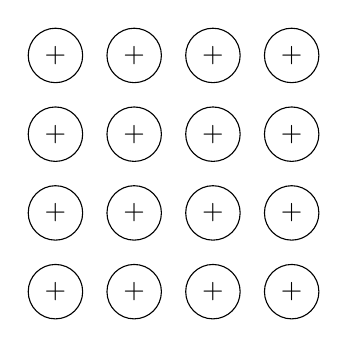
\begin{tikzpicture}
		\foreach \x in {1, 2, 3, 4}
			\foreach \y in {1, 2, 3, 4}
				\node[draw, circle] at (\x, \y) {$+$};
	\end{tikzpicture}

	A metal

	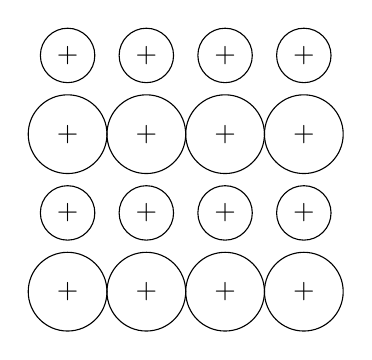
\begin{tikzpicture}
		\foreach \x in {1, 2, 3, 4} {
			\foreach \y in {1, 3}
				\node[draw, circle, minimum size=10mm] at (\x, \y) {$+$};
			\foreach \y in {2, 4}
				\node[draw, circle, minimum size=4mm] at (\x, \y) {$+$};
		};

	\end{tikzpicture}

	An alloy\footnote{These diagrams are far too bad to be acceptable answers to O-Level questions,
	please refer to prescribed book.}
\end{center}

\subsection{Reactivity series}
As shown at the beginning of the chapter, the order of reactivity of the metals is:
$$\underbrace{\ce {K} > \ce{Na} > \ce{Ca} > \ce{Mg} > \ce{Al}}_\text{high reactivity}>
\ce{C} > 
\underbrace{\ce{Zn} > \ce{Fe} > \ce{Pb}}_\text{moderate reactivity} > \ce{H} > 
\underbrace{\ce{Cu} > \ce{Ag} > \ce{Au}}_\text{low reactivity}
$$

The reactivity of a metal is said to be the tendency of the metal to form a positive ion. The 
relative reactivity of each metal is seen in displacement reactions involving the metals, where
the more reactive metal displaces the less reactive metal from its compound. An example follows,
where $\Lambda$ is a more reactive metal than $\Pi$.

\begin{center}
	\ce{$\Lambda$ + $\Pi$SO4 -> $\Pi$ + $\Lambda$SO4}
\end{center}
Note that, the less reactive metal is reduced and the more reactive metal is oxidised. The 
reactions of metals with water, hydrochloric acid and steam have all been discussed, some further
observations are given below.

Potassium, sodium and calcium have very strong reactions with cold water, where the potassium and
calcium are seen to skip over the water's surface while melting. Calcium reacts strongly. Magnesium,
only reacts with cold water very slowly, but burns with a brilliant flame when steam is passed over
heated magnesium.

Metals which are highly reactive have very violent reactions with dilute acid, so it is unsafe to
add them directly. 

Magnesium reacts strongly, disappearing into the acid while forming bubbles of
gas. The result is a colourless solution.

Aluminium is slow to react in cold acid, but bubbles form on heating, causing the aluminium to
disappear into the acid resulting in a colourless solution.

Zinc, disappears in cold acid, producing bubbles of gas and a colourless solution forms. Same is
the case with iron, only a pale green solution is formed.

Copper silver and gold, i.e., metals with low reactivity have no reaction with acids at all.

Aluminium, when kept exposed to air, reacts with the surrounding oxygen in the air resulting in
a layer of aluminium oxide around the sample of aluminium. This layer is unreactive, so aluminium
is \textit{apparently} unreactive as the layer is non porous and no oxygen can reach the 
underlying aluminium.

Given a set of experimental observations, using the strength of reactions described and the 
knowledge from the reactivity series of metals, we can deduce the reactivity of given metals.

\subsection{Corrosion of metals}
Metals corrode under certain conditions as results of certain reactions.

Iron and steel corrode in presence of oxygen or water producing a layer of iron (III) oxide, called
rust. Prevention of this comes down to many strategies, including barrier protection, where the
metal is either coated by another or painted so as to prevent contact of water and oxygen with the
metal. Barriers used to protect metals from corrosion can be painting, greasing or coating the
metal with plastic.

Sacrificial protection consists of another more reactive metal being placed adjacent the metal
to be protected. The moisture and air will then react with the more reactive metal in precedence to
the relatively less reactive metal. In other words, the higher reactive metal loses electrons more
readily, as a result, that metal is oxidised and the lower reactive metal is not corroded.

The two strategies can be combined in that zinc can be used to electroplate any metal, where since
zinc is more reactive, it will be reduced in precedence to the metal being coated. The disadvantage
to barrier protection is that when the coating comes off, that area will immediately be corroded.
This method prevents that as even if the layer is scratched, the moisture will react with the zinc
instead. This method is called galvanising.

\subsection{Extraction of metals}
Metals can be extracted easily depending on their reactivity.

Iron is found naturally in an ore called haematite, which is iron (III) oxide. Iron is extracted
from iron (III) oxide in a blast furnace, by means of reduction by carbon monoxide.

Raw materials, iron ore, coke (carbon made from coal) and the mineral\footnote{A naturally ocurring
rock containing a particular compound} limestone. The furnace has blasts of hot air sent near
the bottom, allowing a series of chemical reactions to occur resulting in the production of pure
iron.

Firstly, the coke burns in the air blast and the furnace gets very hot from this exothermic
reaction:
$$ \ce{C + O2 -> CO2} $$
As carbon dioxide rises through the furnace it reacts with more carbon and is reduced to carbon
monoxide:
$$ \ce{CO2 + C -> 2CO} $$
The most important reaction is the reduction of haematite by this carbon monoxide
$$ \ce{Fe2O3 + 2CO -> 2Fe + CO2} $$
This produced iron flows to the bottom of the furnace where it can be tapped off.

Iron ore contains the impurity sand, which is silicon (IV) oxide, also called silica. Limestone,
calcium carbonate
is added to the blast furnace to rid the iron of this impurity. Firstly, the calcium carbonate
decomposes in the heat of the furnace:
$$ \ce{CaCO3 -> CaO + CO2} $$
Subsequently, this calcium oxide reacts with silica to form calcium silicate, also called slag.
$$ \ce{SiO2 + CaO -> CaSiO3} $$

Aluminium is a metal that shows high reactivity, as a result reduction cannot be used for its 
extraction, rather, electrolysis is employed.

Cryolite is used as a solvent for aluminium as it reduces the melting point of the substance 
allowing the mixture to be liquid at lower temperatures which is economical. It also conducts
electricity and as a result can be used in electrolysis.

The ore for aluminium is bauxite, which is simply aluminium oxide.

Bauxite, dissolved in cryolite is electrolysed using carbon electrodes. The cathode reactions
are as follows:
\begin{center}
	at cathode: \ce{Al^{3+}(l) + 3e- -> Al(l)}

	at anode: \ce{2O^{2-}(l) -> O2(g) + 4e-}
\end{center}

At the very high temperature of the electrolysis conditions, the oxygen being formed at the anode
burns the carbon in the anode,
$$\ce{C(s) + O2(g) -> CO2(g)}$$
forming carbon dioxide and causing the anodes to corrode and be regularly replaced.


\end{document}
